% !TEX root = ../../ctfp-reader.tex

\lettrine[lhang=0.17]{F}{ree constructions are} a powerful application of adjunctions. A
\newterm{free functor} is defined as the left adjoint to a \newterm{forgetful
functor}. A forgetful functor is usually a pretty simple functor that
forgets some structure. For instance, lots of interesting categories are
built on top of sets. But categorical objects, which abstract those
sets, have no internal structure --- they have no elements. Still, those
objects often carry the memory of sets, in the sense that there is a
mapping --- a functor --- from a given category $\cat{C}$ to
$\Set$. A set corresponding to some object in $\cat{C}$ is called
its \newterm{underlying set}.

Monoids are such objects that have underlying sets --- sets of elements.
There is a forgetful functor $U$ from the category of monoids
$\cat{Mon}$ to the category of sets, which maps monoids to their
underlying sets. It also maps monoid morphisms (homomorphisms) to
functions between sets.

I like to think of $\cat{Mon}$ as having split personality. On the one
hand, it's a bunch of sets with multiplication and unit elements. On the
other hand, it's a category with featureless objects whose only
structure is encoded in morphisms that go between them. Every
set-function that preserves multiplication and unit gives rise to a
morphism in $\cat{Mon}$.

Things to keep in mind:

\begin{itemize}
\tightlist
\item
  There may be many monoids that map to the same set, and
\item
  There are fewer (or at most as many as) monoid morphisms than there
  are functions between their underlying sets.
\end{itemize}

\begin{figure}[H]
\centering
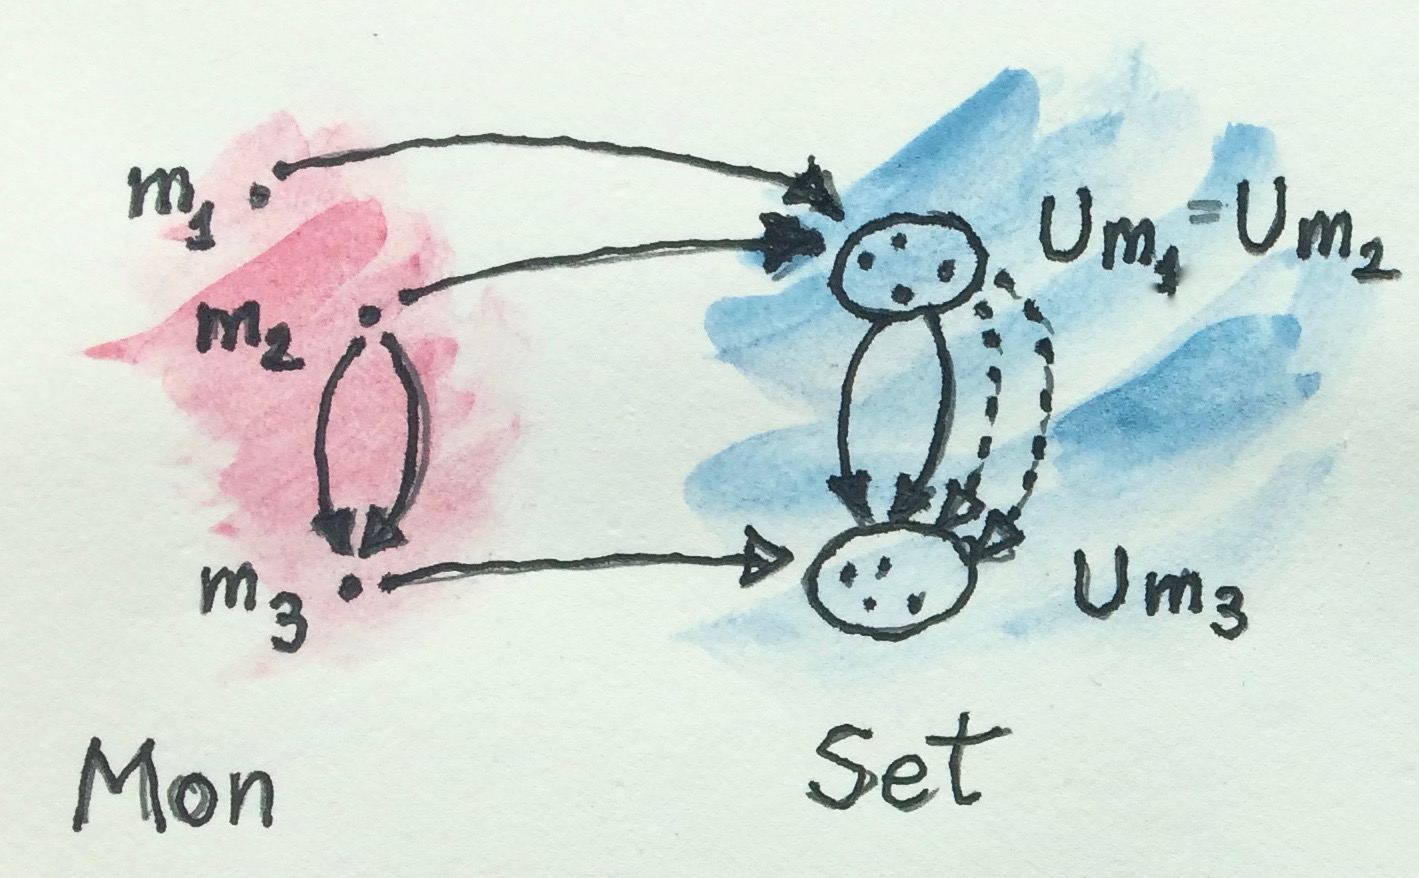
\includegraphics[width=80mm]{images/forgetful.jpg}
\caption{Monoids $m_1$ and $m_2$ have the same
underlying set. There are more functions between the underlying sets of
$m_2$ and $m_3$ than there are morphisms
between them.}
\end{figure}

\noindent
The functor $F$ that's the left adjoint to the forgetful functor
$U$ is the free functor that builds free monoids from their
generator sets. The adjunction follows from the free monoid
universal construction we've discussed before.\footnote{See ch.13 on
\hyperref[free-monoids]{free monoids}.}

In terms of hom-sets, we can write this adjunction as:
\[\cat{Mon}(F x, m) \cong \Set(x, U m)\]
This (natural in $x$ and $m$) isomorphism tells us that:

\begin{itemize}
\tightlist
\item
  For every monoid homomorphism between the free monoid $F x$
  generated by $x$ and an arbitrary monoid $m$ there is a
  unique function that embeds the set of generators $x$ in the
  underlying set of $m$. It's a function in
  $\Set(x, U m)$.
\item
  For every function that embeds $x$ in the underlying set of
  some $m$ there is a unique monoid morphism between the free
  monoid generated by $x$ and the monoid $m$. (This is the
  morphism we called $h$ in our universal construction.)
\end{itemize}

\begin{figure}[H]
\centering
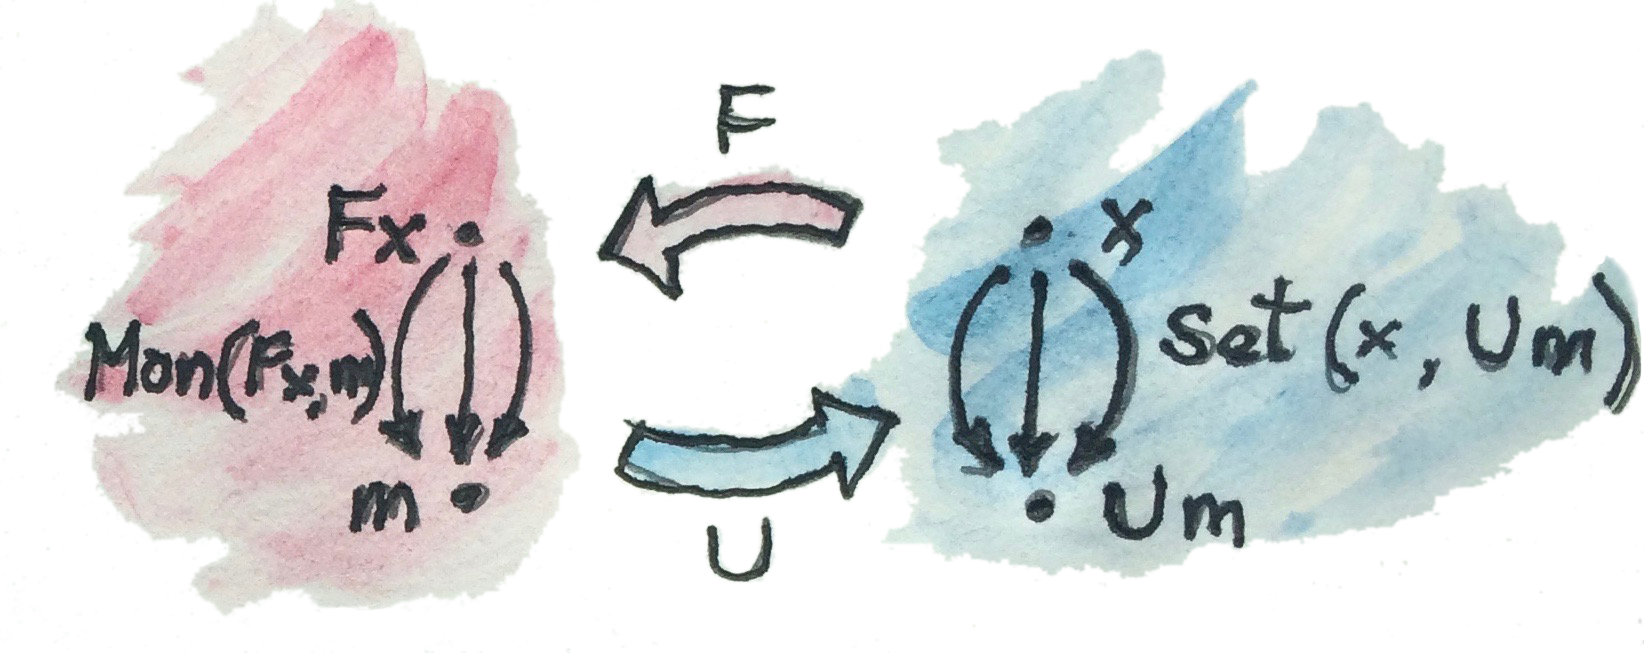
\includegraphics[width=\textwidth]{images/freemonadjunction.jpg}
\end{figure}

\noindent
The intuition is that $F x$ is the ``maximum'' monoid that can
be built on the basis of $x$. If we could look inside monoids, we
would see that any morphism that belongs to $\cat{Mon}(F x, m)$
\emph{embeds} this free monoid in some other monoid $m$. It does
it by possibly identifying some elements. In particular, it embeds the
generators of $F x$ (i.e., the elements of $x$) in
$m$. The adjunction shows that the embedding of $x$, which
is given by a function from $\Set(x, U m)$ on the right,
uniquely determines the embedding of monoids on the left, and vice
versa.

In Haskell, the list data structure is a free monoid (with some caveats:
see \urlref{http://comonad.com/reader/2015/free-monoids-in-haskell/}{Dan
Doel's blog post}). A list type \code{{[}a{]}} is a free monoid with
the type \code{a} representing the set of generators. For instance,
the type \code{{[}Char{]}} contains the unit element --- the empty
list \code{{[}{]}} --- and the singletons like
\code{{[}'a'{]}}, \code{{[}'b'{]}} --- the
generators of the free monoid. The rest is generated by applying the
``product.'' Here, the product of two lists simply appends one to
another. Appending is associative and unital (that is, there is a
neutral element --- here, the empty list). A free monoid generated by
\code{Char} is nothing but the set of all strings of characters from
\code{Char}. It's called \code{String} in Haskell:

\src{code/haskell/snippet01.hs}
(\code{type} defines a type synonym --- a different name for an
existing type).

Another interesting example is a free monoid built from just one
generator. It's the type of the list of units, \code{{[}(){]}}. Its
elements are \code{{[}{]}}, \code{{[}(){]}}, \code{{[}(), (){]}},
etc. Every such list can be described by one natural number --- its
length. There is no more information encoded in the list of units.
Appending two such lists produces a new list whose length is the sum of
the lengths of its constituents. It's easy to see that the type
\code{{[}(){]}} is isomorphic to the additive monoid of natural
numbers (with zero). Here are the two functions that are the inverse of
each other, witnessing this isomorphism:

\src{code/haskell/snippet02.hs}
For simplicity I used the type \code{Int} rather than
\code{Natural}, but the idea is the same. The function
\code{replicate} creates a list of length \code{n} pre-filled with a
given value --- here, the unit.

\section{Some Intuitions}

What follows are some hand-waving arguments. Those kind of arguments are
far from rigorous, but they help in forming intuitions.

To get some intuition about the free/forgetful adjunctions it helps to
keep in mind that functors and functions are lossy in nature. Functors
may collapse multiple objects and morphisms, functions may bunch
together multiple elements of a set. Also, their image may cover only
part of their codomain.

An ``average'' hom-set in $\Set$ will contain a whole spectrum of
functions starting with the ones that are least lossy (e.g., injections
or, possibly, isomorphisms) and ending with constant functions that
collapse the whole domain to a single element (if there is one).

I tend to think of morphisms in an arbitrary category as being lossy
too. It's just a mental model, but it's a useful one, especially when
thinking of adjunctions --- in particular those in which one of the
categories is $\Set$.

Formally, we can only speak of morphisms that are invertible
(isomorphisms) or non-invertible. It's that latter kind that may be
thought of as lossy. There is also a notion of mono- and epi- morphisms
that generalize the idea of injective (non-collapsing) and surjective
(covering the whole codomain) functions, but it's possible to have a
morphism that is both mono and epi, and which is still non-invertible.

In the Free ⊣ Forgetful adjunction, we have the more constrained
category $\cat{C}$ on the left, and a less constrained category $\cat{D}$
on the right. Morphisms in $\cat{C}$ are ``fewer'' because they have to
preserve some additional structure. In the case of $\cat{Mon}$, they
have to preserve multiplication and unit. Morphisms in $\cat{D}$ don't
have to preserve as much structure, so there are ``more'' of them.

When we apply a forgetful functor $U$ to an object $c$ in
$\cat{C}$, we think of it as revealing the ``internal structure'' of
$c$. In fact, if $\cat{D}$ is $\Set$ we think of $U$
as \emph{defining} the internal structure of $c$ --- its
underlying set. (In an arbitrary category, we can't talk about the
internals of an object other than through its connections to other
objects, but here we are just hand-waving.)

If we map two objects $c'$ and $c$ using $U$,
we expect that, in general, the mapping of the hom-set
$\cat{C}(c', c)$ will cover only a subset of
$\cat{D}(U c', U c)$. That's because morphisms in
$\cat{C}(c', c)$ have to preserve the additional structure,
whereas the ones in $\cat{D}(U c', U c)$ don't.

\begin{figure}[H]
\centering
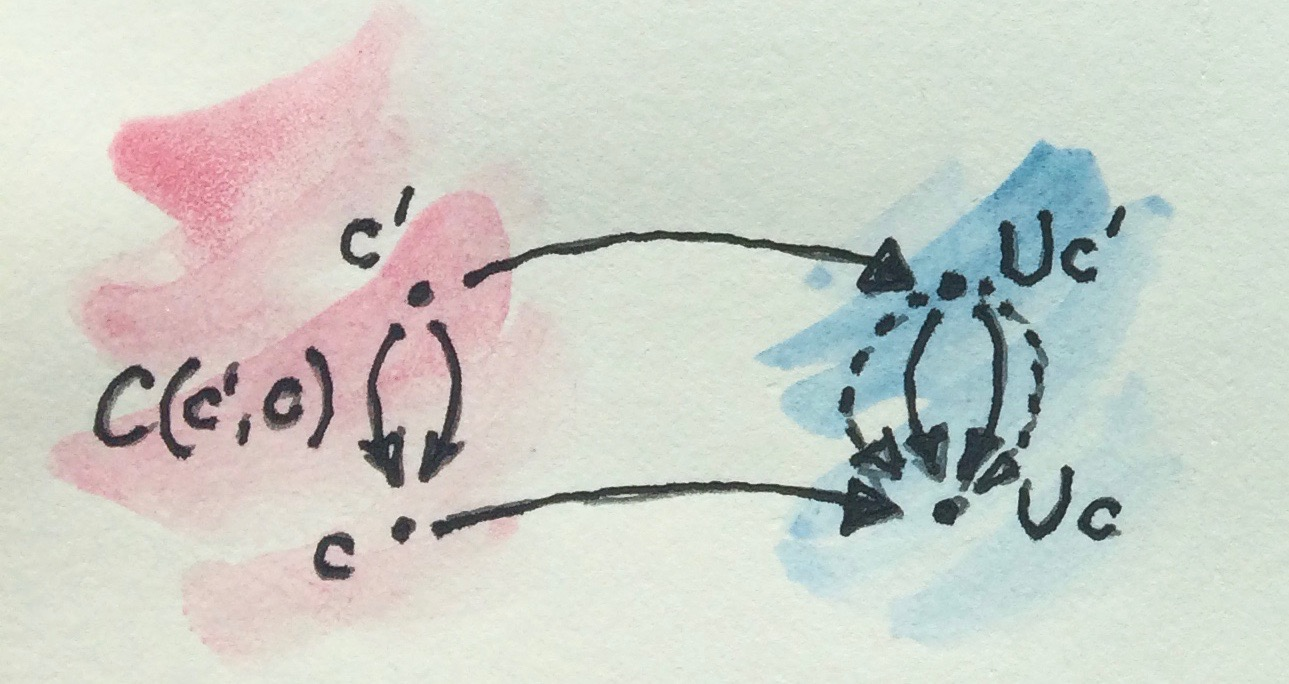
\includegraphics[width=60mm]{images/forgettingmorphisms.jpg}
\end{figure}

\noindent
But since an adjunction is defined as an \newterm{isomorphism} of
particular hom-sets, we have to be very picky with our selection of
$c'$. In the adjunction, $c'$ is picked not
from just anywhere in $\cat{C}$, but from the (presumably smaller) image
of the free functor $F$:
\[\cat{C}(F d, c) \cong \cat{D}(d, U c)\]
The image of $F$ must therefore consist of objects that have lots
of morphisms going to an arbitrary $c$. In fact, there has to be
as many structure-preserving morphisms from $F d$ to $c$
as there are non-structure preserving morphisms from $d$ to
$U c$. It means that the image of $F$ must consist of
essentially structure-free objects (so that there is no structure to
preserve by morphisms). Such ``structure-free'' objects are called free
objects.

\begin{figure}[H]
\centering
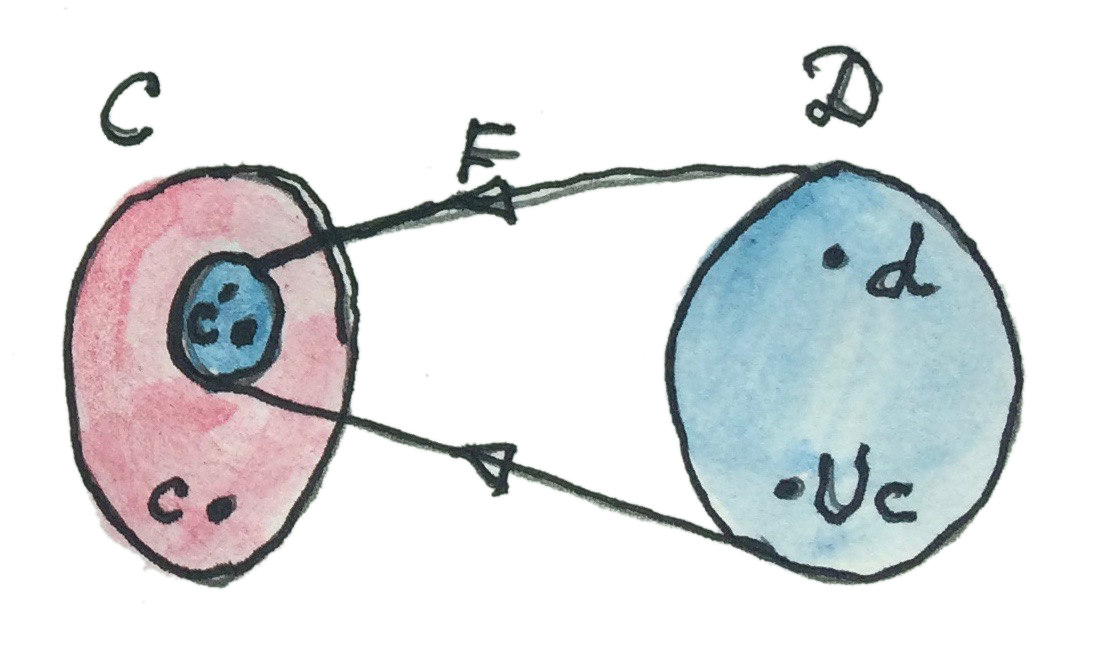
\includegraphics[width=60mm]{images/freeimage.jpg}
\end{figure}

\noindent
In the monoid example, a free monoid has no structure other than what's
generated by unit and associativity laws. Other than that, all
multiplications produce brand new elements.

In a free monoid, $2 * 3$ is not $6$ --- it's a new element ${[}2, 3{]}$. Since
there is no identification of ${[}2, 3{]}$ and $6$, a morphism from this
free monoid to any other monoid $m$ is allowed to map them
separately. But it's also okay for it to map both ${[}2, 3{]}$ and $6$
(their product) to the same element of $m$. Or to identify ${[}2,
3{]}$ and $5$ (their sum) in an additive monoid, and so on. Different
identifications give you different monoids.

This leads to another interesting intuition: Free monoids, instead of
performing the monoidal operation, accumulate the arguments that were
passed to it. Instead of multiplying $2$ and $3$ they remember $2$ and $3$ in a
list. The advantage of this scheme is that we don't have to specify what
monoidal operation we will use. We can keep accumulating arguments, and
only at the end apply an operator to the result. And it's then that we
can chose what operator to apply. We can add the numbers, or multiply
them, or perform addition modulo 2, and so on. A free monoid separates
the creation of an expression from its evaluation. We'll see this idea
again when we talk about algebras.

This intuition generalizes to other, more elaborate free constructions.
For instance, we can accumulate whole expression trees before evaluating
them. The advantage of this approach is that we can transform such trees
to make the evaluation faster or less memory consuming. This is, for
instance, done in implementing matrix calculus, where eager evaluation
would lead to lots of allocations of temporary arrays to store
intermediate results.

\section{Challenges}

\begin{enumerate}
\tightlist
\item
  Consider a free monoid built from a singleton set as its generator.
  Show that there is a one-to-one correspondence between morphisms from
  this free monoid to any monoid $m$, and functions from the
  singleton set to the underlying set of $m$.
\end{enumerate}
